\documentclass[conference]{IEEEtran}
\IEEEoverridecommandlockouts
% The preceding line is only needed to identify funding in the first footnote. If that is unneeded, please comment it out.

\usepackage[T1]{fontenc}
\usepackage[utf8]{inputenc}
\usepackage{lmodern}

\usepackage{cite}
\usepackage{amsmath,amssymb,amsfonts}
\usepackage{algorithmic}
\usepackage{graphicx}
\usepackage{textcomp}
\usepackage{xcolor}
\usepackage{url}
\usepackage{datetime}
\usepackage{microtype}

\newdateformat{schoolyear}{%
  \ifthenelse{\month > 9} % If current month is October or later
    {\the\year/\the\numexpr\year+1-2000\relax} % Show current year / next year (last two digits)
    {\the\numexpr\year-1\relax/\the\numexpr\year-2000\relax} % Show previous year / current year (last two digits)
}

\def\BibTeX{{\rm B\kern-.05em{\sc i\kern-.025em b}\kern-.08em
    T\kern-.1667em\lower.7ex\hbox{E}\kern-.125emX}}
\usepackage{parskip}





\begin{document}

\title{Assignment \#X:\\My Fantastic Approach for Something}

\author{

\IEEEauthorblockN{Name Surname}
\IEEEauthorblockA{\textit{IBB \schoolyear\today, FRI, UL} \\
    \textit{your.email@you.use.as.an.email.id}}
% \and
% \IEEEauthorblockN{Second Author}
% \IEEEauthorblockA{\textit{IBB 22/23, FRI, UL} \\
%     \textit{your.email@you.use.as.an.email.id}}

}

\maketitle

\begin{abstract}
Abstract is intended for final paper at project-oriented track. When writing it, please follow instructions that were given during lab sessions. For assignments feel free to omit the abstract.
\end{abstract}

% ########################################
\section{Introduction}
Write some short introduction.

% ########################################
\section{Related Work}
Briefly overview other works and do not forget to cite~\cite{someexample2019} them. To export nicely formatted citations Google Scholar usually works the best (select export bib).

% ########################################
\section{Methodology}
Describe what you have done -- without experimental specifics (without actual numbers or data).

% ########################################
\section{Experiments}
How the experiments looked like, what data was used (and some properties), what were the parameters used, etc.

% ########################################
\section{Results and Discussion}
Short sentence here.

% #################
\subsection{Results}
Include tables and figures here, do not forget to reference them in the text, such as Table~\ref{tab1} and Fig.~\ref{fig1} and emphasize important bits.

\begin{table}[h]
\caption{Table description -- explain what the table shows.}
\begin{center}
\begin{tabular}{llll}
 A [\%]&  B [\%]&  C [\%]&  D [\%]  \\
 \hline
 99&  99&  99&  99  \\
 99&  99&  99&  99 
\end{tabular}
\label{tab1}
\end{center}
\end{table}

\begin{figure}[b]
\begin{center}
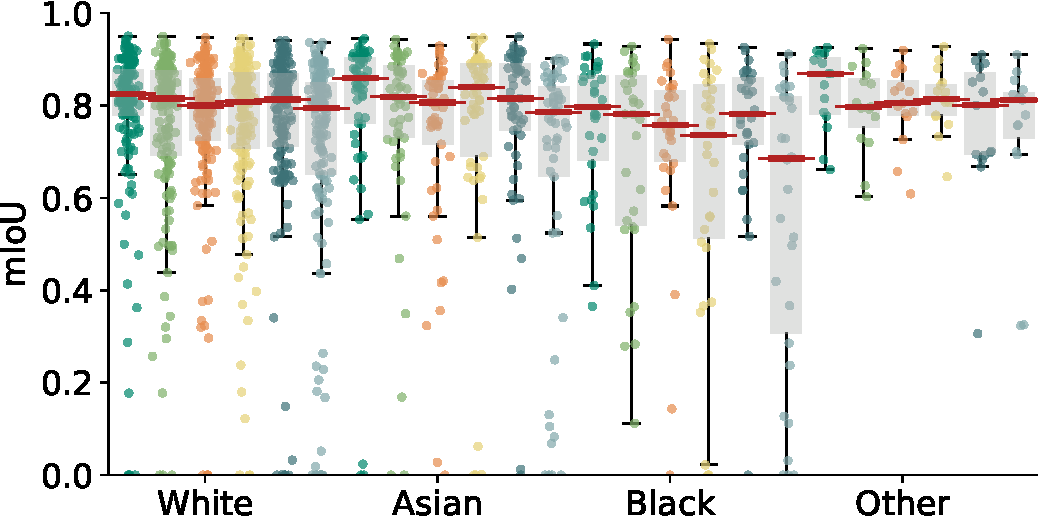
\includegraphics[width=0.9\columnwidth]{figs/example_plot.pdf}
\end{center}
\caption{Figure caption -- be long here -- this should stand on its own, without the need to read the rest of the text.}
\label{fig1}
\end{figure}

% #################
\subsection{Discussion}
Try to explain the results and why you think something is as it is.

% ########################################
\section{Conclusion}
Conclude the work and summarize your findings.

% ########################################
\bibliographystyle{IEEEtran}
\bibliography{report}

\end{document}
